\documentclass[preprint,12pt]{article}

\usepackage{algorithmic}
\usepackage{algorithm}
\usepackage{enumerate}
\usepackage{enumitem}
\usepackage{graphics}
\usepackage{graphicx}
\usepackage{geometry}
\usepackage{amsmath}
\usepackage{wrapfig}
\usepackage{subfig}
\usepackage{framed}
\usepackage{color}
\usepackage{soul}
\usepackage{bm}

\usepackage{multirow}
\usepackage[T1]{fontenc}
\usepackage[latin9]{inputenc}
%\usepackage{units}
\usepackage{esint}

\geometry{legalpaper,  margin=1in}

\newcommand{\CM}[2][green]{ {\sethlcolor{#1} \hl{#2}} }
\newcommand{\KB}[2][cyan]{ {\sethlcolor{#1} \hl{#2}} }

%\makeatother

%\usepackage{babel}fs

\begin{document}
\title{Extracting the components of Specific Partisan Asymmetry for Wisconsin Assembly 2010 census cycle districts}
\author{Kevin Baas and Colin McAuliffe}
\maketitle
\begin{abstract}
The changes in partisan asymmetry in the Wisconsin state assembly legislative maps from the 2000 census cycle to the 2010 census cycle are analyzed using an empirical Bayesian method.
The 2010 map is found to increase the number of seats won by Republicans compared to the 2000 map, and to increase the partisan asymmetry by almost exactly the same number of seats.
The increased bias in the 2010 cycle election results is therefore primarily the result of redistricting, and there is no evidence that natural political geography or changes in voter preferences can explain the changes in bias.
\end{abstract}

\section{Method}

\begin{figure}[htb!]
    \begin{center}
        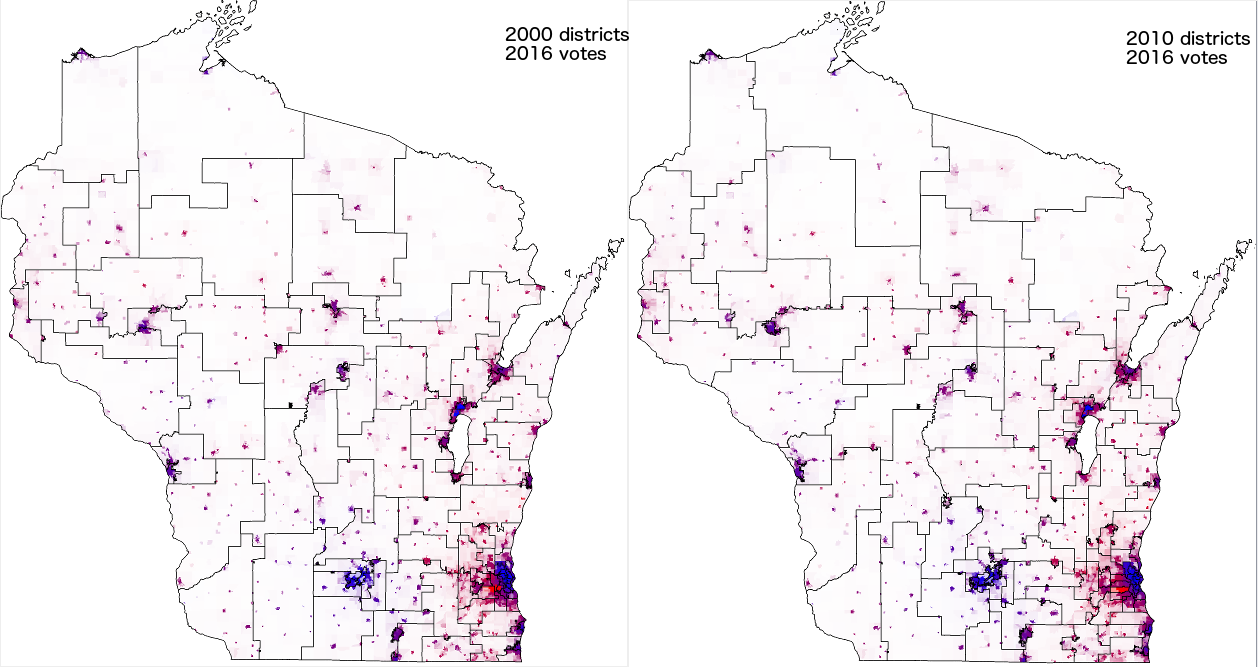
\includegraphics[scale=0.35]{../Figures/WI_compared/precincts_pop_combined.png}
        \caption{2016 Assembly election results by precinct, projected onto Assembly districts before and after Act 43. Left: 2000 cycle districts, Right: 2010 cycle districts}\label{fig:Maps}
    \end{center}
\end{figure}

To compare how much of the observed partisan asymmetry in 2010-cycle Wisconsin State Assembly districts was the result of changes in district designs versus changes in voter sentiment, we varied the first while holding the second constant.
In other words, we projected actual election results onto both the current Assembly districts, and Assembly districts from the previous redistricting cycle, as shown in figure \ref{fig:Maps}.

For this analysis we used official districting plans for the 2000 and 2010 census cycles, and actual vote counts from the 2006, 2008, 2010, 2012, 2014, and 2016 assembly elections, at precinct-level resolution, imputing uncontested elections with partisan swing matched presidential election results when available, and partisan swing matched federal congress election results when not.
By "partisan swing matched" we mean that the Republican vote counts in all districts are multiplied by a constant factor so that the total vote count matches that for the assembly elections, for the subset of districts in which both elections were contested, and the same is done for the Democratic vote counts.
Then election data for 2006, 2008, and 2010 was cross-aggregated at census block resolution to the 2010-cycle districts, and election data for 2012, 2014, and 2016 was cross-aggregated at census block resolution to the 2000-cycle districts. 
 
Since the same exact elections are used in both the 2000 districts analysis and 2010 districts analysis, \emph{all} differences in the results are the consequence of the redistricting scheme used, and conversely, changes in voter sentiment have exactly \emph{zero} contribution to the difference.

Furthermore, if the 2000 census cycle districts show a partisan asymmetry much lower than the 2010 cycle, then we know that natural "political geography" -- the tendency of Democratic voters to be clustered in cities -- can be immediately ruled out as a significant factor in the partisan asymmetry inherent in 2010 cycle Wisconsin Assembly districts, since any contributions from political geography would be present in \emph{both} districting schemes.
However if they are not substantially different, this would not demonstrate that political geography was a significant contribution, because they both could be artificially gerrymandered on top of any unintentional gerrymandering due to political geography.
In this case, further analysis would be required to separate the effects of unintentional bias caused by political geography and deliberate bias caused by gerrymandering.

\section{Measurement}
To measure partisan bias, we measured the asymmetry in the seats-votes curve at the actual vote count that occurred in the election.  
In other words, we take the number of seats that Republicans won, and subtract from that the number of seats that Democrats would have won if the popular vote percentage was reversed (1-x), and divide by 2.  
This represent the number of seats Republicans won in excess of what they would have won if the seats-votes curve was symmetric.  
If the number is negative, that represents an asymmetry in favor of Democrats.
We call this "specific partisan asymmetry".

Before applying this metric to concrete examples, we'd like to highlight some of the advantages of it.

\begin{itemize}

\item It doesn't assume proportionality in results - The seats-votes curve for single-winner elections naturally take on a cumulative Beta-binomial distribution, as opposed to a diagonal line representing seats proportional to votes.  This metric doesn't assume a diagonal curve representing proportionality.  It tests a looser (less strict) criteria: asymmetry, which still retains the essential feature of measuring disenfranchisement based on political belief.  SCOTUS has ruled that seats proportional to votes can not be a legal standard (Thornburg v. Gingles 1986).   But they remain open to a legal standard based on the idea of partisan symmetry (LULAC v. Perry 2004).
 
\item It distinguishes between artificial partisan bias and the natural multiplying effect of single-winner elections -  Single-winner aka "Majoritarian" elections naturally over-favor the majority party, giving them a larger fraction of the seats than they get of the popular vote.  
While some measures might mistakenly identify this as gerrymandering, specific asymmetry explicitly takes this into account by calculating and then subtracting this natural multiplying effect.
In other words, it does not mistake disproportionality due to the sigmoidal shape of majoritarian election seats-votes curves with gerrymandering.

\item It works for states with partisanship far from 50/50 - By sampling the asymmetry at the actual vote counts rather than e.g. 50/50, this metric maintains full relevance even for the most extremely partisan states.

\item It represents deviation from what is practically achievable - It is trivial for a computer algorithm to design districts that make the seats-votes curve perfectly symmetric, while satisfying all constitutional requirements.  
Thus, to convert this absolute score to one relative to what can be accomplished by a redesign that meets all traditional redistricting principles, one simply subtracts zero.  
This "new" relative score gives you the number of voters whose votes were effectively stolen by the map drawers with the current map, and whose right to representation can be returned by a remedy map that can be trivially designed by a computer employing a multi-objective heuristic optimization algorithm.

\item The only possible improvements to it are shift, scale, and shape - Since it is well ordered and monotonic with respect to actual partisan advantage, any "better" measure can only be better in the sense of having a more appropriate "center" point, a more appropriate scale, or a more appropriate "shape" (change of slope as you go up and down the scale).  The scale varies from -1 to 1, or alternatively from negative the number of seats available to the positive of that.  The "center",  zero, is a non-arbitrary and very reasonable choice, representing a perfectly symmetric situation.   The "shape" is the number (or percentage) of congressional seats affected.

\item It gives a result in an empirically meaningful unit: number of seats, which can be directly converted into number of ballots/voters affected by multiplying by the number of ballots cast and dividing by the number of districts.

\end{itemize}


\section{Observed partisan asymmetries in past elections}

\begin{figure}[htb!]
    \begin{center}
        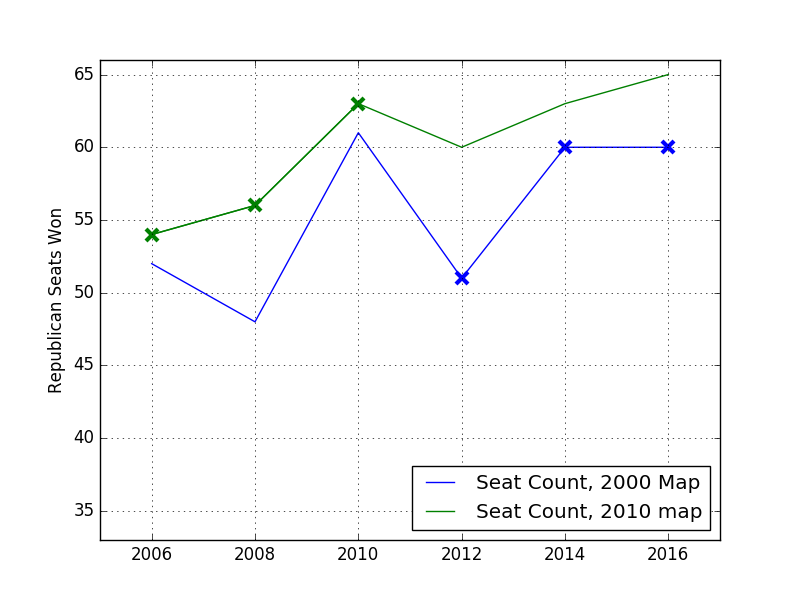
\includegraphics[scale=0.85]{../Figures/WI2010/WI_2000_2010_seats.png}
        \caption{Republican Seat Counts in Assembly elections, using 2000 cycle districts vs 2010 cycle districts. The X's indicate that a result has been cross aggregated, meaning results were computed on a different district map than the one that actually existed at the time of the election}\label{fig:Seats20002010}
    \end{center}
\end{figure}

\begin{figure}[htb!]
    \begin{center}
        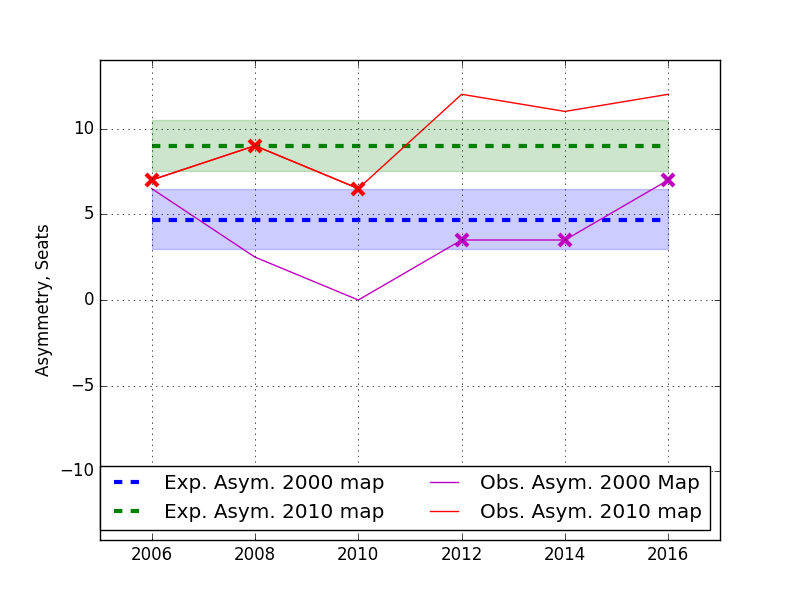
\includegraphics[scale=0.85]{../Figures/WI2010/WI_2000_2010.png}
        \caption{Historical asymmetry in Assembly elections, using 2000 cycle districts vs 2010 cycle districts. The X's indicate that a result has been cross aggregated, meaning results were computed on a different district map than the one that actually existed at the time of the election}\label{fig:Asym20002010}
    \end{center}
\end{figure}

After imputing uncontested elections and projecting onto the two different districting schemes, we counted up the wins for each election on each map.
We also counted up the wins for the other party if the popular vote was reversed, subtracted this from the first, and divided by 2, to get the specific partisan asymmetry.
The seat counts are shown in figure \ref{fig:Seats20002010}, and the specific asymmetry is shown in figure \ref{fig:Asym20002010}.  They are also tabulated in table \ref{tab:seats}.
The horizontal lines and shaded regions represent the statistical expectation and 50\% confidence intervals, respectively.
Their calculation is described in the next section.

The charts show a clear and stable separation between both seat counts and partisan asymmetry between 2000 districts and 2010 districts.
They both go up and down largely in parallel, responding about the same to changes in voter sentiment.

This tells us that in the 2012, 2014, and 2016 elections, the new districts led to an increase in Republican representation over what the old districts would have produced.
Furthermore, were the new districts used in the 2000 redistricting cycle, that would have produced about the same increase in Republican representation for the 2006, 2008, and 2010 elections.

\begin{table}[htb!]
\centering
\caption{Summary of the differences in seat counts and asymmetries for elections on the two legislative maps \label{tab:seats}}
\begin{tabular}{|l|l|l|l|}
\hline
Election Year & Rep. Seats, 2000 Map & Rep. Seats, 2010 Map & Net Change in Seats\\
\hline
\hline
2006 & 52 & 54 & R + 2\\
\hline
2008 & 48 & 56 & R + 8\\
\hline
2010 & 61 & 63 & R + 2\\
\hline
2012 & 51 & 60 & R + 9\\
\hline
2014 & 60 & 63 & R + 3\\
\hline
2016 & 60 & 65 & R + 5\\
\hline
\hline
Election Year & Asymmetry, 2000 Map & Asymmetry, 2010 Map & Net Change in Asymmetry\\
\hline
\hline
2006 & 6.5 & 7.0 & R + 0.5\\
\hline
2008 & 2.5 & 9.0 & R + 6.5\\
\hline
2010 & 0.0 & 6.5 & R + 6.5\\
\hline
2012 & 3.5 & 12.0 & R + 8.5\\
\hline
2014 & 3.5 & 11.0 & R + 7.5\\
\hline
2016 & 7.0 & 12.0 & R + 5.0\\
\hline
\end{tabular}
\end{table}


In figure \ref{fig:Asym20002010diff}, the difference in seats won by Republicans is plotted along with the difference in the expected asymmetries between the two maps.
The increase in seats gained by Republicans in the 2010 map is entirely explained by the increase in asymmetry in the 2010 map.
Therefore the 2010 map leads to greater Republican representation by \emph{structurally disadvantaging Democratic voters}.


\begin{figure}[htb!]
    \begin{center}
        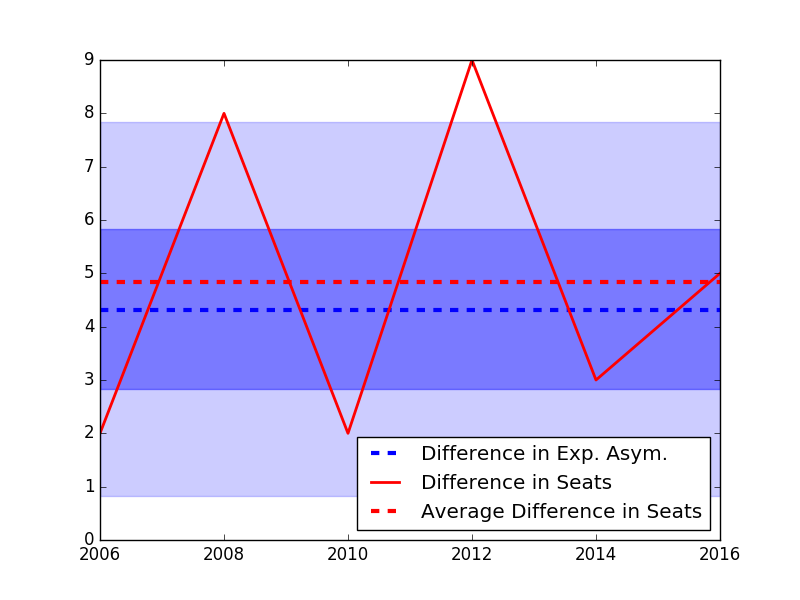
\includegraphics[scale=0.85]{../Figures/WI2010/WI_2000_2010diff.png}
        \caption{Difference in seats won by Republicans in the two maps. The dashed blue line shows the difference in expected asymmetry between the two maps, the blue and light blue shaded regions represent 50\% and 90\% confidence intervals}\label{fig:Asym20002010diff}
    \end{center}
\end{figure}

\begin{figure}[htb!]
    \begin{center}
        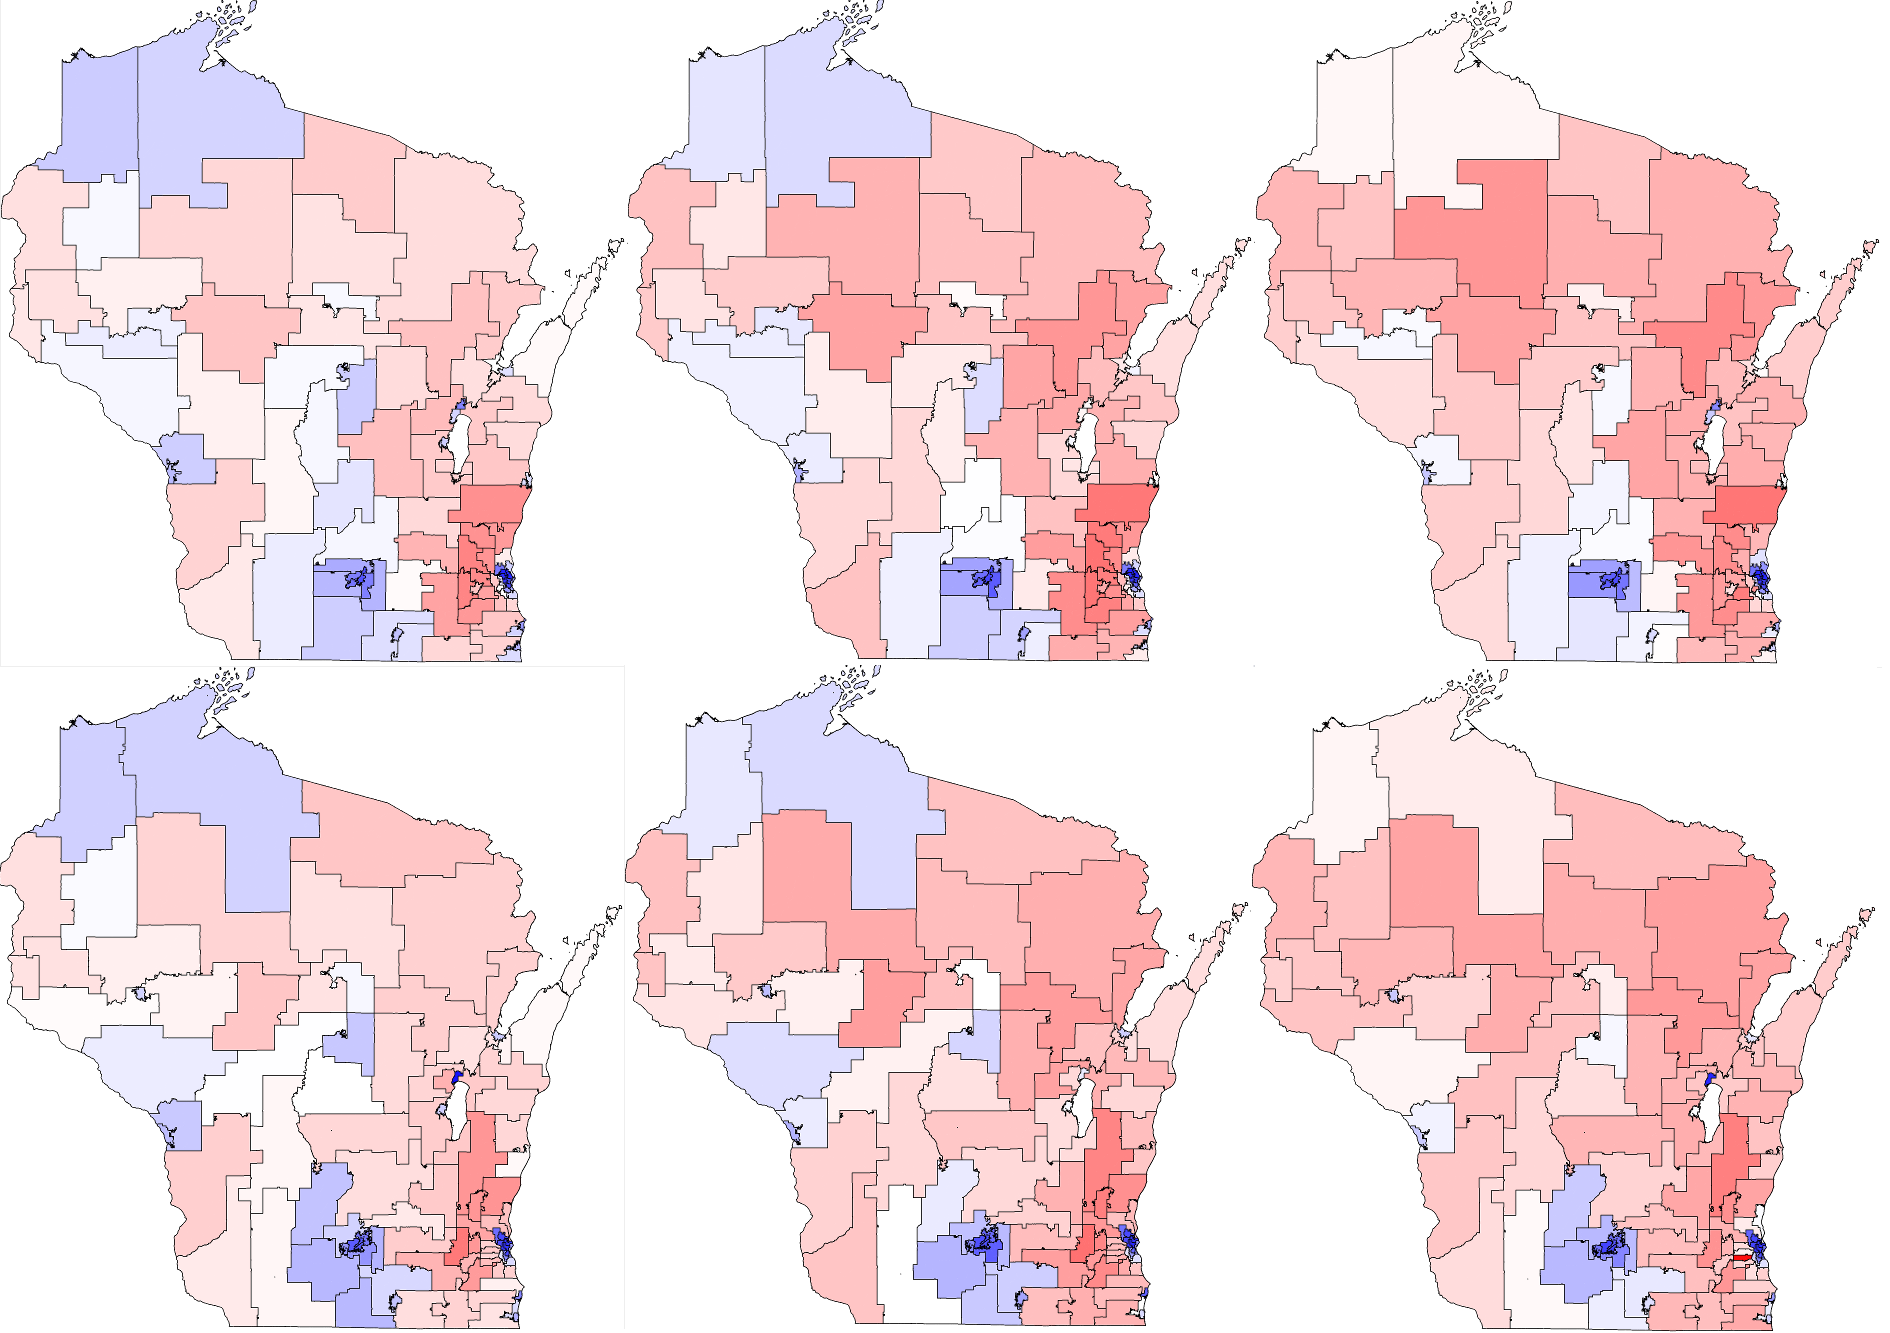
\includegraphics[scale=0.25]{../Figures/WI_compared/3x2.png}
        \caption{Partisan vote packing in Wisconsin Assembly elections. Top: 2000 cycle districts, Bottom: 2010 cycle districts, Left to right: 2012, 2014, and 2016 elections}\label{fig:DistrictMaps}
    \end{center}
\end{figure}


We can better visualize how the 2010 districts give Republicans more seats than the 2000 districts by coloring in the districts according to the victory margin, and comparing.
Figure \ref{fig:DistrictMaps} shows such a comparison for 2012, 2014, and 2016 elections (left to right).
The two Democratic districts above Lake Winnebago were combined into one, thus taking a seat away from Democrats.
Democratic voters in Eau Claire once participated in two competitive districts, which would have given Democrats 2 seats with 2000 district lines, but the 2010 district lines wrapped them up in a single safe district, capping the number of elections those voters can swing at 1.
In 2000 districts, Madison is surrounded by a bunch of competitive Democratic-leaning districts.
But the 2010 lines packed Democratic voters surrounding Madison into a few safe Democratic districts, flipping the districts those voters came from, which would have been competitive, to Republican.
In Milwaukee, the lines were redrawn to more tightly outline Democratic voters, thus creating a few more districts that Republicans can win in.
Indeed, figure \ref{fig:DistrictMapDelta} shows that by comparing the districting schemes using 2016 votes, it is easy to identify where Republicans picked up 4 seats due to partisan vote packing.

Meanwhile, deeper red districts throughout the state were redrawn to give away some of their Republican voters to nearby competitive districts,
thus reducing the likelihood that a Democratic representative was elected in the once-competitive districts,
while still maintaining a safe edge in the originally deeper red district.  
You can see this by noticing the much "flatter" red color in the bottom maps versus the top maps.
It will also be made clear in the next section when we examine the statistical properties of the maps more rigorously.

In sum, the changes in the district lines from 2000 districts to 2010 districts consist of packing Democratic voters, thus decreasing the number of Democratic districts, and cracking Republican districts, thus increasing their number.
Instances of the reverse -- of packing Republican voters and cracking Democratic districts -- are simply not present.
\begin{figure}[htb!]
    \begin{center}
        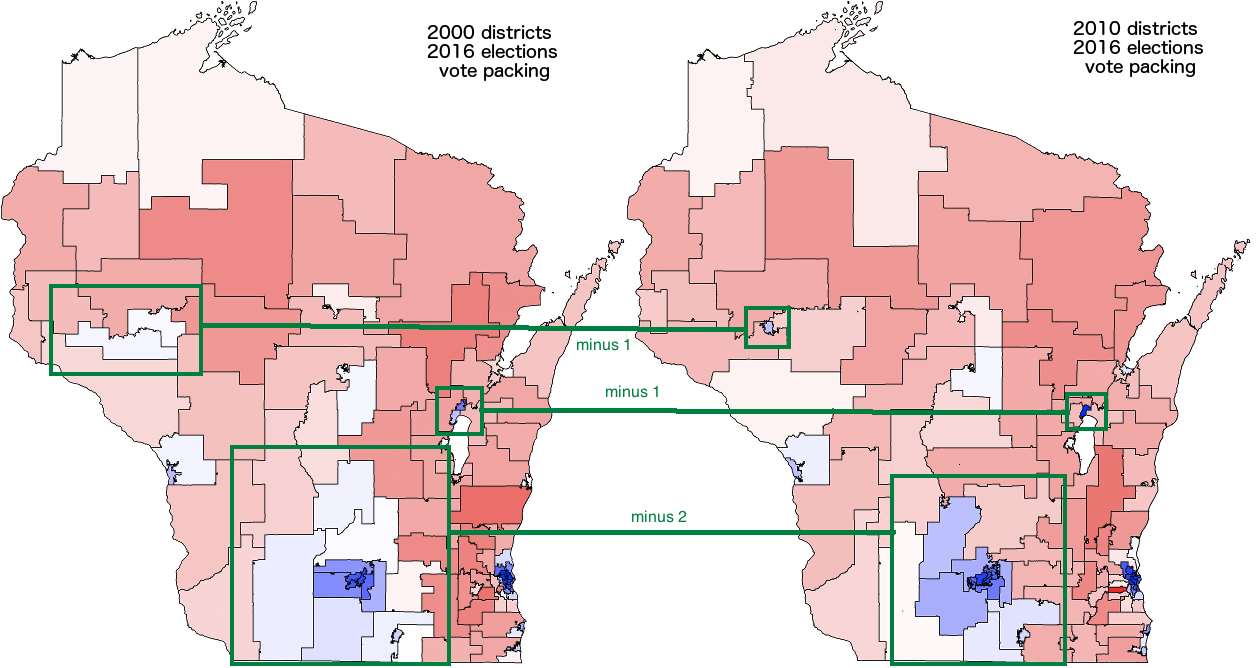
\includegraphics[scale=0.40]{../Figures/WI_compared/districts_compared_deltas.png}
        \caption{Partisan vote packing in Wisconsin Assembly elections, using 2016 election data.  Outlined in green are areas where Republicans packed Democratic votes.}\label{fig:DistrictMapDelta}
    \end{center}
\end{figure}



\section{Expected  partisan asymmetries in future elections}

\subsection{Probability model}

To calculate the expected partisan asymmetries for future elections, we need to construct a probability model and compute the most likely parameters for it based on past observations.
We choose our probability model by deduction from first principles.

An election between two parties is a number of repeated trials, each resulting in one of two outcomes.  This is known in mathematical literature as a Bernoulli process.
In our case, the rate of "success" (of getting the first of the two options) in the Bernoulli process -- known as the "rate parameter" -- is unknown.
For reasons which we won't go into here, the standard accepted distribution for modeling an unknown rate parameter of a Bernoulli process, is a Beta distribution.
Using a Beta distribution here amounts to making the fewest possible assumptions about the value of the rate parameter.

For our probability model we model at the resolution of districts vote percentages.
We use a Beta distribution for the vote counts in each district, and one for the total popular vote.
Thus we empirically estimate a probability model that represents the entire range of plausible outcomes for the election results under a particular redistricting plan.
Sampling the model allows us to calculate a likelihood for every possible outcome, without relying on any prior assumptions.
We can therefore not only determine the presence of partisan asymmetry in the outcome of one or more election results, but we can determine whether or not and to what degree partisan asymmetry is a persistent feature of a given plan.

Before applying this model to a concrete examples, we'd like to highlight some of the advantages of this approach.

\begin{itemize}

\item It takes into account non-uniform swings - By looking at not only the average partisanship of each district, but how much the partisanship of each individual district changes from election to election, this metric is able to take into account the changes in voter sentiment that are not uniform throughout the state; that are perhaps concentrated in only certain districts.

\item It takes into account all possibilities, weighted by likelihood - Every possible seats-votes curve and every possible popular vote ratio is taken into consideration, weighted by the combined likelihood of the two.

\item It shows durability - By computing an entire likelihood function for specific partisan asymmetry, rather than a single point estimate, this approach enables quick and accurate assessment of how durable a gerrymander is; how much more harm it will cause in the future, including what the likelihood is that it will not cause harm.

\end{itemize}

\subsection{Future election result likelihoods}

\begin{figure}[htb!]
    \begin{center}
        \includegraphics[scale=0.25]{../Figures/WI_compared/Betas_cropped.png}
        \caption{Beta distributions for Wisconsin 2010-cycle Assembly districts, Top: 2000 cycle districts, Bottom: 2010 cycle districts}\label{fig:Betas}
    \end{center}
\end{figure}
 
Shown in figure \ref{fig:Betas} is a graph of district partisanship, including dispersion. 
On top are 2000 cycle districts, and on bottom are 2010 cycle districts.   
To generate this graph, a Beta distribution for each district was calculated using the method of moments.  Additionally a Beta distribution for the total popular vote was calculated using the method of moments.  Then the probability density function was plotted out for each one of them (The black curve in the middle is the total popular vote.)
Results that lead to a Democrat winning the seat are colored in blue, and results that lead to a Republican winning the seat are colored in red.
Note, in addition to the average of the past 6 elections, the graph also shows the statistical dispersion, from which the durability of this effect for future elections can be assessed.

Both the 2000 and 2010 distributions show clear signs of pro-Republican gerrymandering: many Republican-leaning districts are tightly clustered at levels of partisanship that allow Republican candidates to win safely without wasting too many votes, while many Democrat-leaning districts are heavily packed and not competitive.
However, in the 2010 distributions Republicans-leaning districts are more concentrated around a single point slightly but safely short of competitive, while Democratic-leaning districts that were competitive in the 2000 distributions have been shifted away from the center.
Consequently, in the 2010 distributions, compared to the 2000 distributions, Republicans are expected to gain more seats by smaller margins, while Democrats are expected to gain fewer seats by larger margins.

Shown in figures \ref{fig:SVAssembly2000} and \ref{fig:SVAssembly2010} are twelve seats-votes curves drawn from these distributions (solid curve), along with their 2-axis reflection (dashed curve), and a popular vote percentage drawn from the statewide Beta distribution (vertical dotted gray line). 
While a small asymmetry in favor of Republicans is sometimes apparent in the 2000 curves, a large and consistent asymmetry in favor of Republicans is immediately evident in the 2010 curves.

\begin{figure}[htb!]
    \begin{center}
        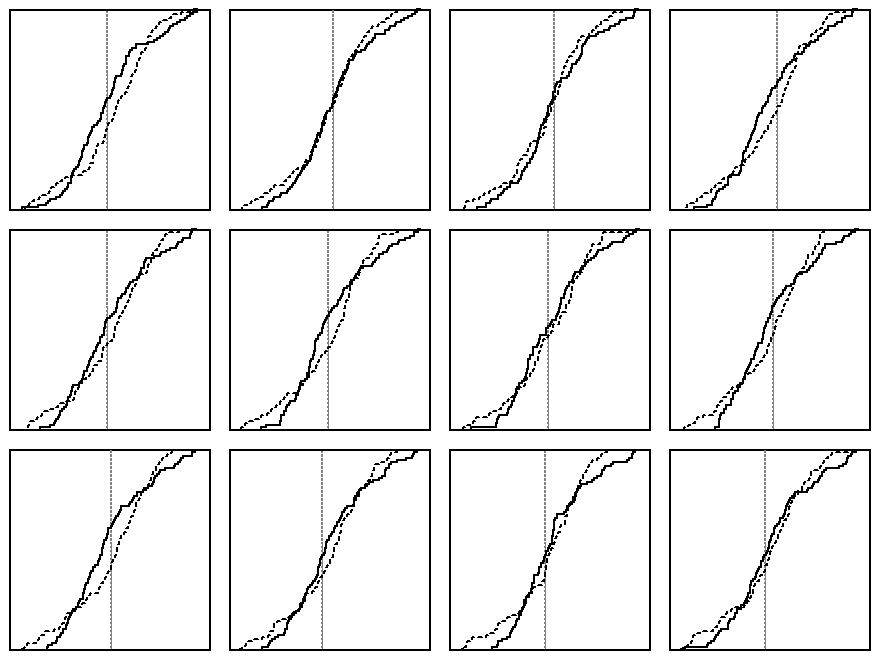
\includegraphics[scale=0.45]{../Figures/WI2000/4x4.png}
        \caption{Some election outcome seats-votes curves generated from the probability model for Wisconsin 2000 Assembly districts}\label{fig:SVAssembly2000}
    \end{center}
\end{figure}
\begin{figure}[htb!]
    \begin{center}
        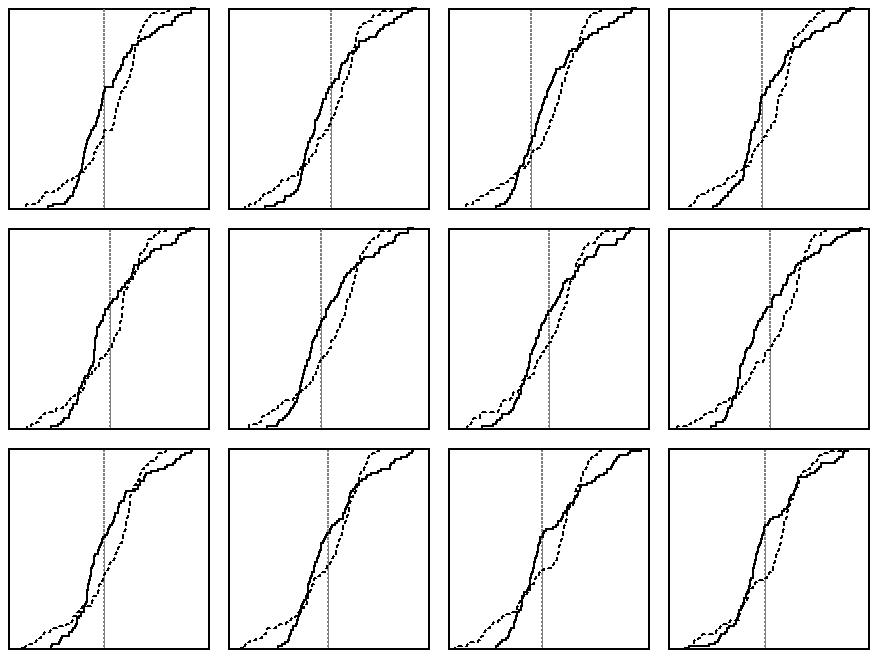
\includegraphics[scale=0.45]{../Figures/WI2010/sv_curves_assembly.png}
        \caption{Some election outcome seats-votes curves generated from the probability model for Wisconsin 2010 Assembly districts}\label{fig:SVAssembly2010}
    \end{center}
\end{figure}

\subsection{Numerical integration of likelihood functions}

\subsubsection{Specific partisan asymmetry likelihoods}
 
To get the likelihood function for partisan asymmetry, we use Monte-Carlo numerical integration.
In each realization, we subtract the seat counts Democrats would get with that share of the vote from the number Republicans would get under the same share of the vote, and then divide by 2. 
The results are shown in figure \ref{fig:LikelihoodsAsymmetry}, as a fraction of total available seats.
 
\begin{figure}[htb!]
    \begin{center}
        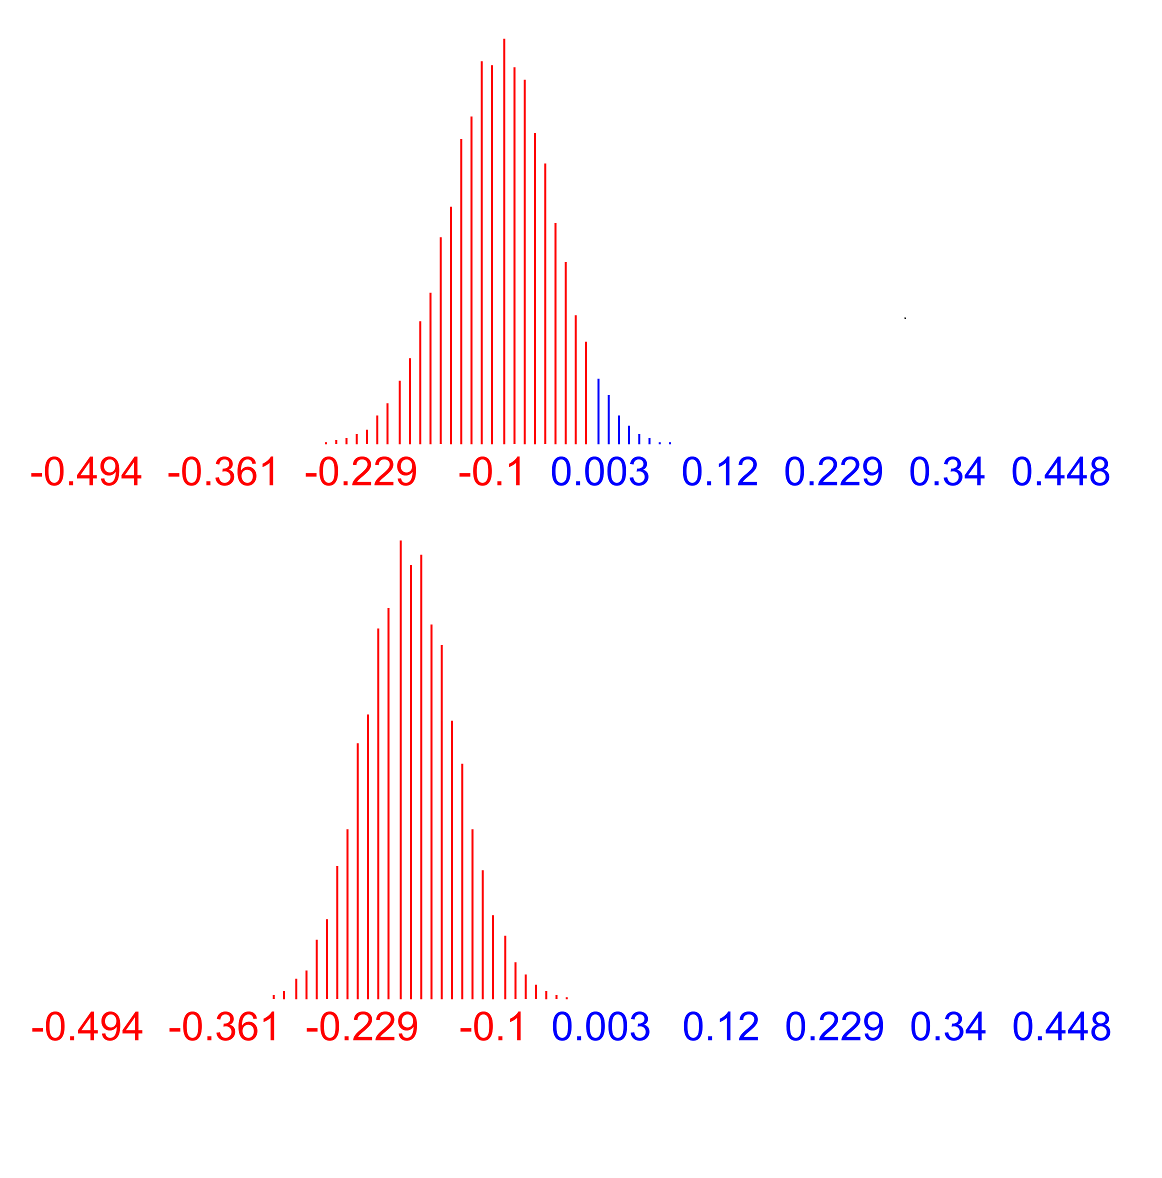
\includegraphics[scale=0.25]{../Figures/WI_compared/asymmetry_cropped.png}
        \caption{Specific asymmetry likelihoods, Top: 2000 cycle districts, Bottom: 2010 cycle districts}\label{fig:LikelihoodsAsymmetry}
    \end{center}
\end{figure}
 
For the 2000 districts, the partisan asymmetry favors Republicans, giving them an average seat boost of 10\% of the available seats beyond what a symmetric seats-votes curve would produce.  
However, there is still a decent likelihood that voter sentiments would change enough that Democrats would get a small boost from seats-votes curve asymmetry.

For the 2010 districts, the partisan asymmetry favors Republicans by twice the amount of the 2000 districts, giving them an average seat boost of 20\% of the available seats beyond what a symmetric seats-votes curve would produce.  
To put this figure in context, we conducted a study of asymmetry in the US federal congress from 1972 to 2016, where we found that asymmetries exceeding 10\% of the available seats were rare and appeared only in the most aggressively gerrymandered states.
The two largest gerrymanders in federal congress in this time period were North Carolina and Pennsylvania in the 2010 cycle, where the asymmetry was about 19\% of the available seats for each of these states.
The most likely result in the Wisconsin state assembly might be that Republicans get 6/10ths of the legislative seats, whereas if the popular vote count were reversed, Democrats would get only 4/10th of the legislative seats.  
Remedying this would give Democrats 10\% more seats.  
This means that roughly 10\% of the entire Democratic-voting population of the state of Wisconsin were effectively disenfranchised, in violation of the one person, one vote principle.  
Conversely, 10\% of the Republican-voting population effectively got an extra vote.  That's approximately 306,000 felonies.

Unlike the 2000 districts, out of 100,000 samples drawn, \emph{none} of them resulted in specific partisan asymmetry favoring Democrats.  
Since an assembly district election occurs every 2 years, this shows that, without significant changes in geo-spatial demographics, the asymmetric pro-Republican partisan advantage inherent in this redistricting will persist for the next 200,000 years.

\subsubsection{District partisanship histogram}
  
\begin{figure}[htb!]
    \begin{center}
        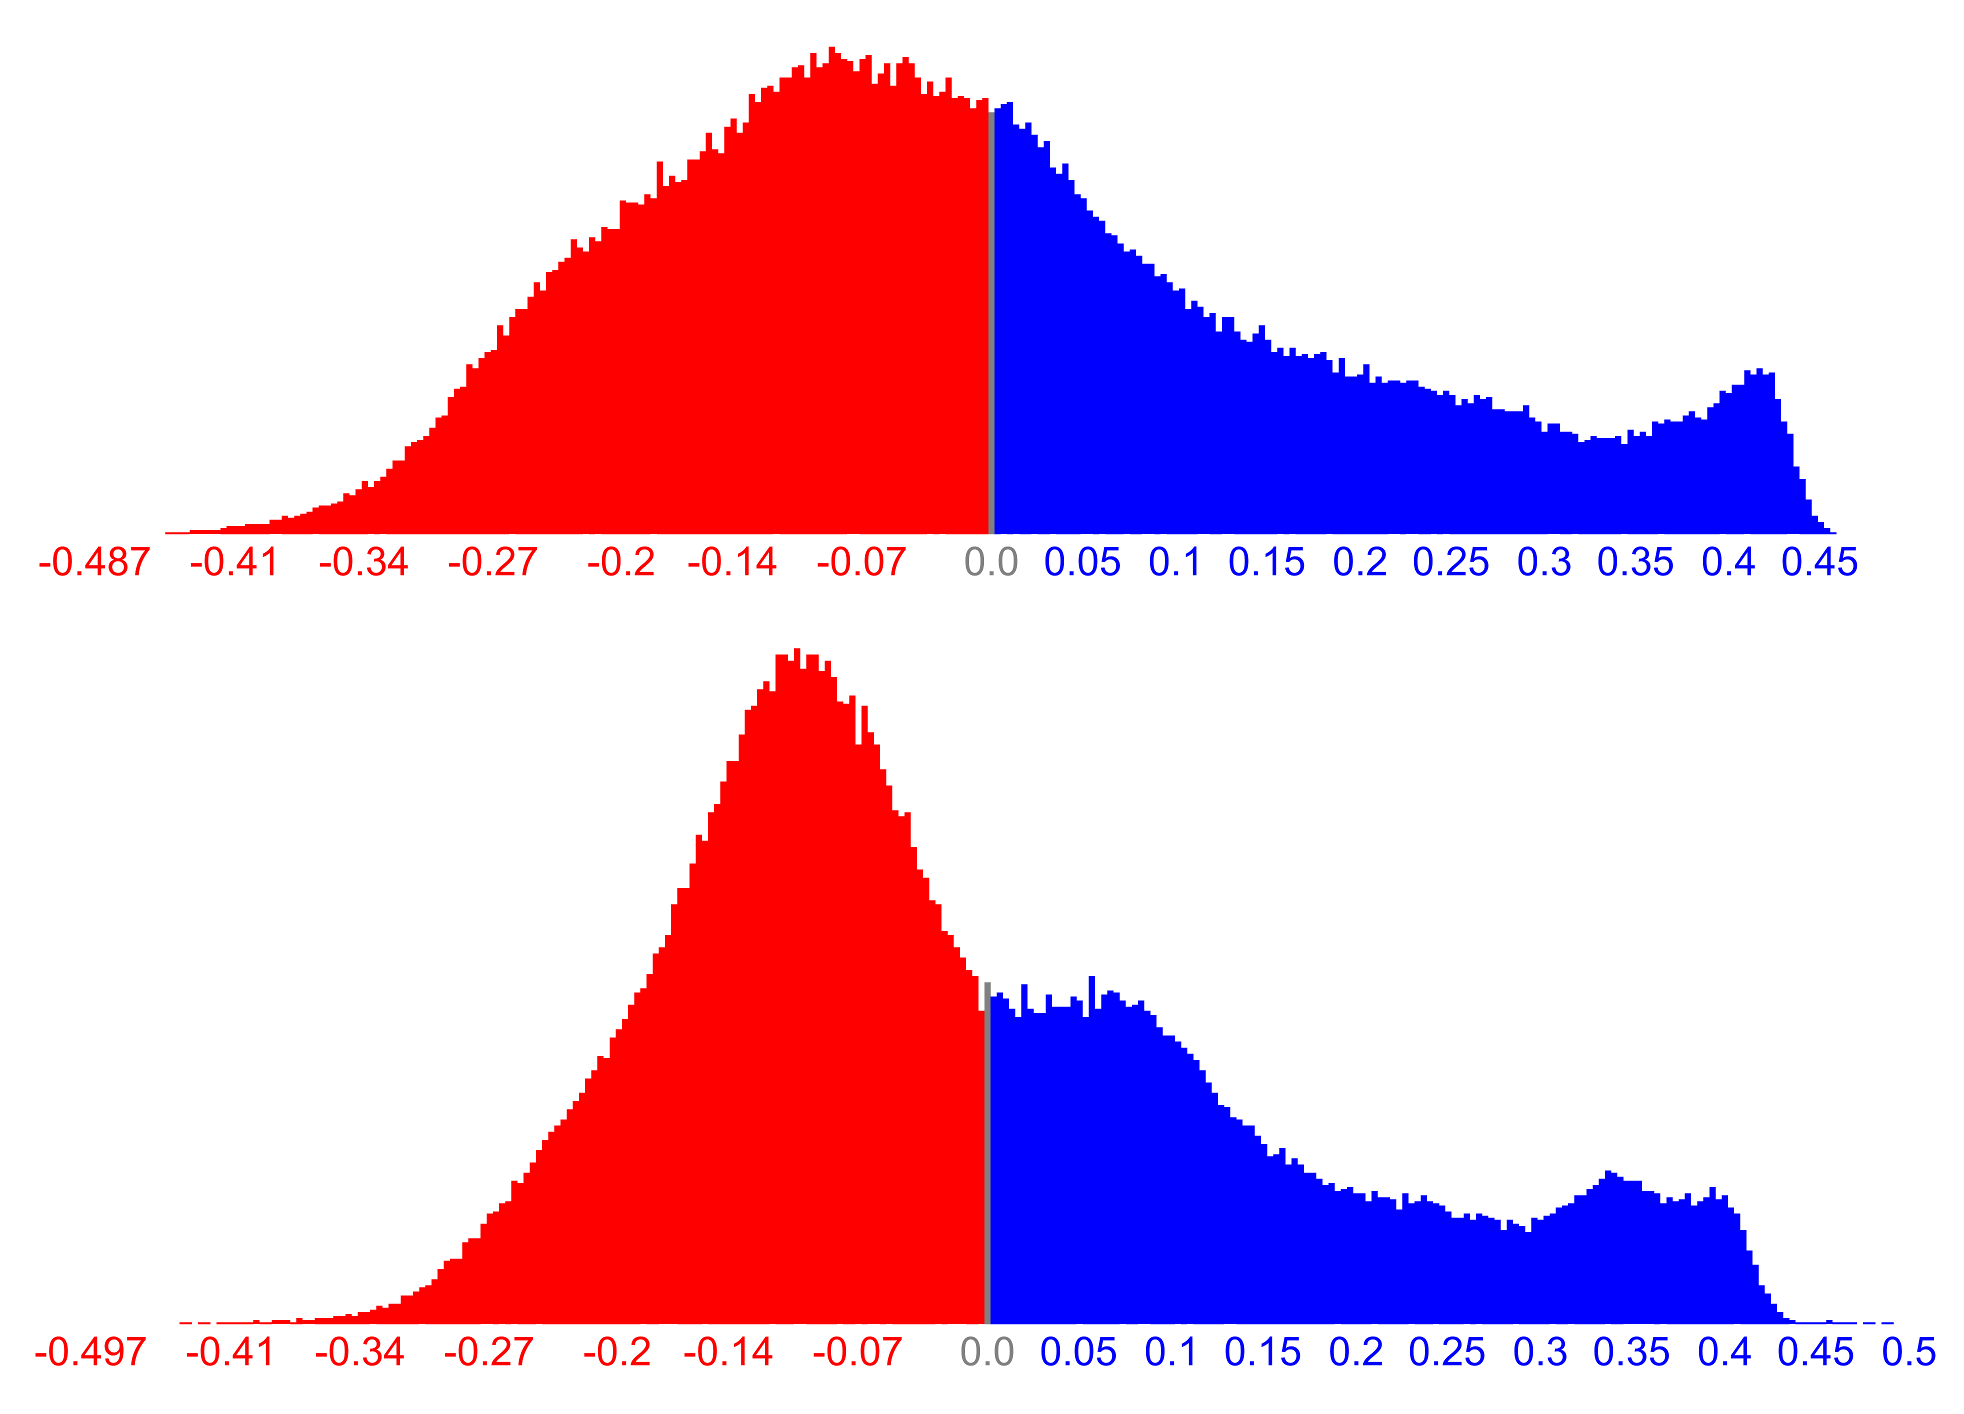
\includegraphics[scale=0.25]{../Figures/WI_compared/district_partisanship_cropped.png}
        \caption{District partisanship likelihoods, Top: 2000 cycle districts, Bottom: 2010 cycle districts}\label{fig:LikelihoodsDistrictPartisanship}
    \end{center}
\end{figure}

Another way we can see this is by looking at the histogram of district partisanship.
 
We used Monte Carlo integration to construct the likelihood function for district partisanship, over all districts, and all possible election outcomes.
In other words, if you were to pick a random district in a random election, this curve shows how likely the vote in that district is to be 25\% Republican vote, a 50-50 split, etc.
This is essentially what you'd see if you took the lines in figure \ref{fig:Betas}, and stacked then on top of each other instead of behind each other. 
 
The curve for the 2000 districts show a smooth peak near 50/50, with a slight skew towards Republicans and a long tail on the Democratic side with a brief peak at the end.  
This shows that Democratic districts were packed, while Republican districts were cracked.

On the other hand the curve for the 2010 districts show a much sharper distinction.
It has a high red peak close to the center but still safely to the side, that already drops off sharply by the time it hits 50/50, and then on the blue side, drops slowly all the way until it gets to a larger bump at the extremely packed end of the scale.
This clearly reveals that Republican candidates in Republican leaning districts have a high likelihood of winning safely but without wasting too many votes, while Democratic candidates in Democratic leaning districts have a high likelihood winning by margins that waste a lot of votes.
You can also see this effect visually on the maps in figure \ref{fig:DistrictMaps}: the red colors are much "flatter" in 2010 districts (bottom) than 2000 districts (top).

\subsubsection{Statewide seat count likelihoods}

\begin{figure}[htb!]
    \begin{center}
        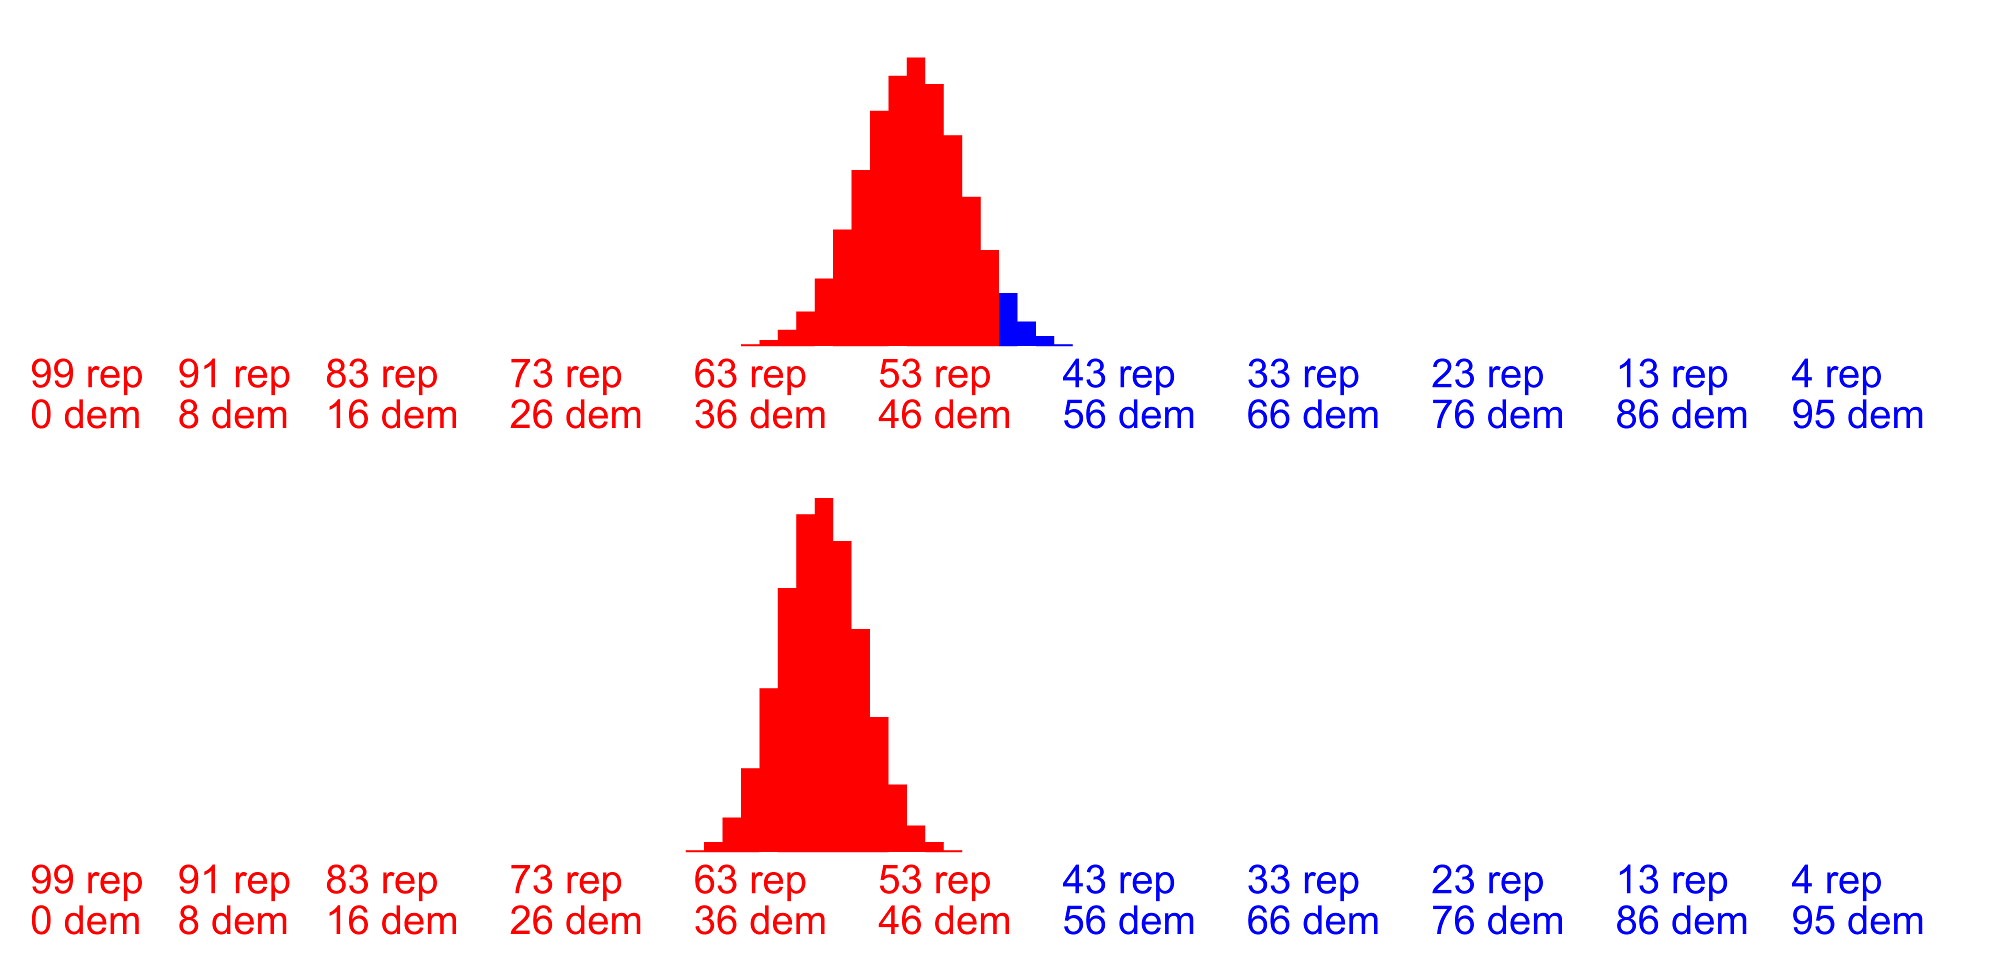
\includegraphics[scale=0.25]{../Figures/WI_compared/seats_cropped.png}
        \caption{Seat count likelihoods, Top: 2000 cycle districts, Bottom: 2010 cycle districts}\label{fig:LikelihoodsSeatCounts}
    \end{center}
\end{figure}
 
Using "draws" from the Beta distributions as shown in figures \ref{fig:SVAssembly2000} and \ref{fig:SVAssembly2010}, we estimate the likelihood of every possible election outcome, district-by-district.
We then accumulate these outcomes on a chart, with the seat count on one axis, and the likelihood on the other.  The results are shown in figure \ref{fig:LikelihoodsSeatCounts}.

In 2000 districts, the average outcome -- also known as the "expected" outcome -- is Republicans winning a 54-45 majority of seats, though Democrats still have a decent chance of winning the majority of seats. 

In 2010 districts, Republican's expected lead grows by an additional 10 seats to 59-40, and despite being favored by roughly half the voters, Democrats have no chance at all to win a majority of seats,  even in the most eccentric swings of voter sentiment.
Indeed, out of 100,000 samples, Democrats rarely even get 45 of the seats -- a threshold that, under the 2000 districting scheme, would be their average.

\section{Conclusions}

Measured by partisan asymmetry, both expected and observed, there was substantial gerrymandering in favor of Republicans in the 2000 cycle maps, leading to about 4 extra Republican seats beyond what would be allocated if the seats-votes curve was symmetric.
The current method does not distinguish what part of this gerrymandering was deliberate and what part unintentional, though regardless of the proportion, it is trivial to generate a map without this asymmetry by using one of many well-known optimization algorithms.

If we disregard data that was not available when the 2010 cycle districts were drawn, and use only data from the 2006, 2008, and 2010 elections, we see that with the new redistricting lines, Republicans are expected to gain an additional 4 assembly seats, beyond what the previous (2000 cycle) redistricting lines would have given them.
Note that for every seat Republicans gain, Democrats lose a seat.  
So in terms of seat \emph{difference} gained, it's 8.
Furthermore, this is in addition to the partisan asymmetry already present in the 2000 cycle maps, bringing the expected total seat difference gained over Democrats through partisan asymmetry to 18.

The fact that the 2010 cycle maps have double the partisan asymmetry as the 2000 maps, both expected and observed, demonstrates that regardless of what part of the gerrymandering in the 2000 cycle maps was deliberate, \emph{at least} half of the gerrymandering in the 2010 cycle maps was deliberate.
Regardless of what portion of the remainder is unintentional, a map optimized by a computer algorithm to maximize partisan symmetry could remove almost all of the deliberate gerrymandering, and at least some of the unintentional gerrymandering.

From these comparisons, it is painfully obvious that the specific partisan asymmetry present in the 2010 cycle districts is \emph{not} present in the 2000 cycle districts, even when using vote count data from the exact same elections.  Therefore:
\begin{itemize}

\item The difference between the two schemes is a stable 10\% gain in the Republican seat margin over Democrats.
Since the same exact voter sentiments were used in both analyses, this difference in partisan asymmetry simply cannot be a consequence of changes in voter sentiment.  
Since the only thing that we changed was the districting scheme, all observed differences in partisan asymmetry are purely the result of changing the districting scheme and reflect the choices made by the redistricters and do not reflect changes in political geography.
\item In order to claim that natural political geography was a significant factor in the 2010 cycle district, we would expect to see the exact same asymmetries in the 2000 districts.
To the contrary, partisan asymmetry in 2010 districts is double that of 2000 districts, even after compensating for observed and potential changes in voter sentiment.
\item Claims that the observed partisan bias in 2010 districts is simply a consequence of political geography are categorically false.
\item Claims that the observed partisan bias in 2010 districts is simply a consequence of changes in voter sentiments are categorically false.
\item Simply reverting back to the 2000 census cycle districts would remedy most of the present injustice, as measured in seats affected or ballots affected.
\end{itemize}

This comparison cannot estimate how much deliberate gerrymandering was present in both schemes, nor can it estimate how much of the gerrymandering present in the 2000 districts was deliberate.
However it does prove with absolute certainty that the 2010 districts, under the same elections, give Republicans more seats than the 2000 districts, and that this difference will persist even in the most extreme swings of voter sentiment.

Currently Assembly Republicans have 64 seats, and Democrats have 35.
If the district lines were not changed after the 2010 cycle, and everyone voted the same, 
Republicans would currently have 4 less seats in Wisconsin Assembly, and Democrats would have 4 more, making the count 60-39.
If the district lines were instead optimized to favor neither party -- to have an expected specific partisan asymmetry of zero -- 
Republicans would currently have 9 less seats in Wisconsin Assembly, and Democrats would have 9 more, making the count 55-44.
For comparison, the historical threshold for ruling in favor of plaintiffs on grounds of racial gerrymandering is 1 seat.

\end{document}
